\documentclass[es,practica]{uah}

\tema{V2}
\titulo{Manipulación de imágenes con GIMP}{}

\begin{document}

\titulacion{Grados Informática}
\asignatura{Sistemas Audiovisuales y Aplicaciones Multimedia}{}
\curso{2021/2022} 


\maketitle


\section{Fotomontaje con GIMP}

En esta sesión, realizaremos un fotomontaje, empleando las distintas herramientas que nos ofrece GIMP. Para realizar el fotomontaje, emplearemos 4 fotografías (preferentemente obtenidas con su propia cámara). El fondo lo constituirá una pared, vista de forma oblicua, como en la figura. Utilizaremos también la foto de un cuadro (o similar) visto de frente, que ``colgaremos'' sobre la pared, una foto de exterior, y una fotografía del propio alumno. La figura siguiente muestra de forma esquemática cómo debería quedar la composición. Evidentemente, el trabajo a realizar debe hacerse con imágenes reales.

\begin{figure}[h!]
  \centering
  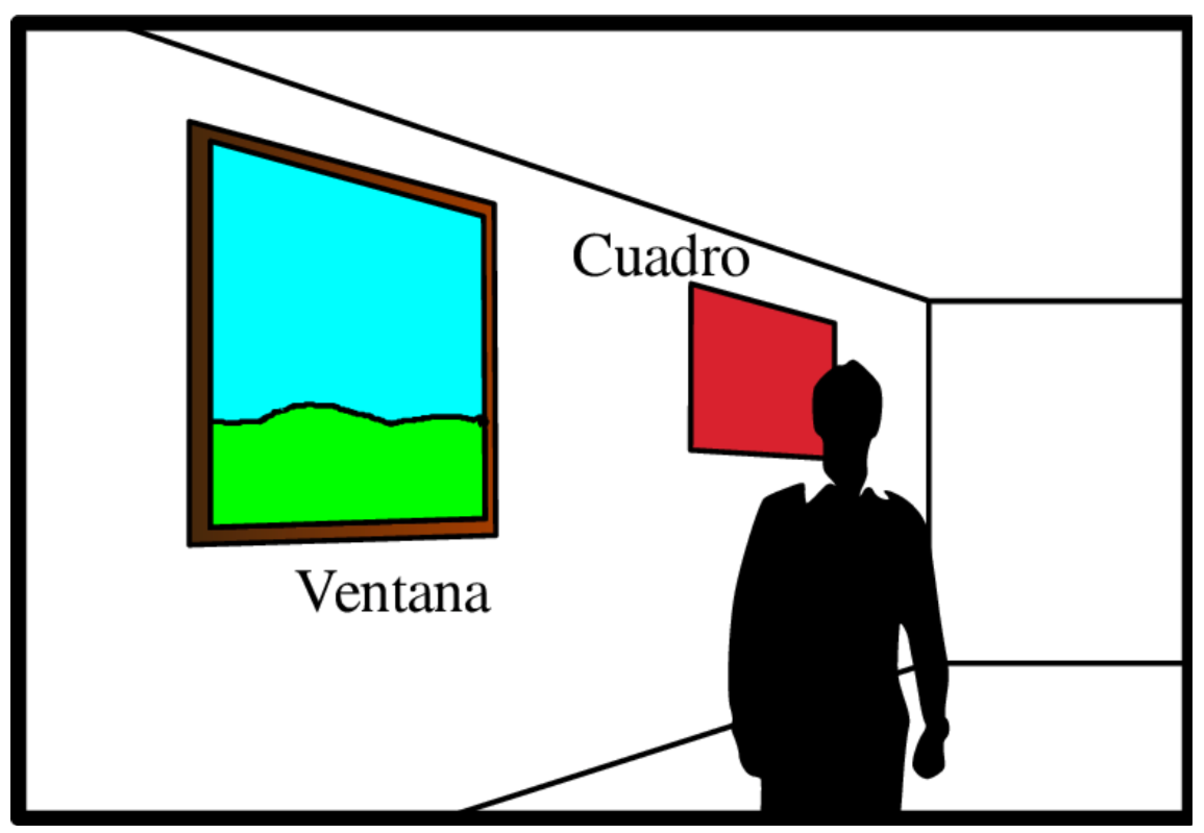
\includegraphics[width=5cm]{Figuras/Figura1}
\end{figure}

Para realizar la composición, abra todas las imágenes como capas, quedando la imagen de exterior debajo, luego la de la habitación, posteriormente el cuadro, y por último la del alumno.

En primer lugar, recortaremos la silueta del alumno. Para ello, puede emplear la herramienta de Tijeras inteligentes del menú Herramientas/Herramientas de selección si el fondo es poco uniforme y los bordes están bien definidos. Por contra, si el fondo es más o menos uniforme, emplee mejor la herramienta de Selección por color, para seleccionar el fondo uniforme, y posteriormente invierta la sección (Seleccionar/Invertir). Para que el resultado sea lo más realista posible, realice una selección difusa, con un radio de unos 3 ó 4 píxeles, para conseguir que los bordes queden ligeramente difuminados. Emplee la máscara rápida para refinar la sección si fuese necesario. Copie y pegue la selección sobre la imagen del fondo, ajustando el tamaño y la posición a conveniencia. Oculte la imagen original del alumno (no la elimine del proyecto).

Posteriormente, ``colocaremos'' el cuadro sobre la pared. Como la pared se visualiza de forma oblicua, necesitamos realizar una transformación de perspectiva. Para realizar la transformación, debemos seleccionar la herramienta de transformación de perspectiva mediante:
\begin{itemize}
	\item Herramientas $\rightarrow$ Herramientas de transformación $\rightarrow$ Perspectiva
\end{itemize}

En este caso, la transformación debe ser hacia adelante, ya que vamos a especificar la zona de la imagen donde se situará el cuadro. Ajuste el método de interpolación a Cúbica.

Para construir la ventana, crearemos un hueco en la imagen que representa la pared. Utilizando la herramienta de Selección libre, hacemos un polígono con la forma de la ventana. Antes de continuar, guardaremos la selección, porque vamos a volver a utilizarla. Para guardar una selección, podemos ejecutar:

\begin{itemize}
	\item Seleccionar $\rightarrow$ A ruta
\end{itemize}

Así mismo, podemos visualizar la nueva ruta mediante:

\begin{itemize}
	\item Ventanas $\rightarrow$ Diálogos empotrables $\rightarrow$ Rutas
	\begin{itemize}
		\item Activamos el icono del ``ojo''
	\end{itemize}
\end{itemize}

Si queremos volver a utilizar una ruta como selección, basta con seleccionar dicha ruta en la ventana anterior y ejecutar:

\begin{itemize}
	\item Seleccionar $\rightarrow$ A partir de una ruta
\end{itemize}


Ocultamos temporalmente la ruta, para proseguir con la ventana. En este caso, tenemos que hacer transparente dicha zona de la capa. No obstante, vamos a darle un toque algo más artístico, realizando el siguiente procedimiento. En primer lugar compruebe si la capa correspondiente a la habitación tiene capa de máscara, mediante:

\begin{itemize}
	\item Capa $\rightarrow$ Máscara $\rightarrow$ Añadir máscara de capa (canal alfa de la capa)
\end{itemize}

Si el comando anterior está habilitado, es porque no tiene máscara de capa. Ejecute dicho comando para añadirla. Si estuviera deshabilitado, no es necesario ejecutar nada. Para trabajar con la transparencia, activamos:

\begin{itemize}
	\item Capa $\rightarrow$ Máscara $\rightarrow$ Mostrar máscara de capa (activar)
	\item Capa $\rightarrow$ Máscara $\rightarrow$ Editar máscara de capa (activar)
\end{itemize}

En este momento, todo lo que editemos se realizará sobre la información de transparencia de la capa, en lugar de sobre la imagen. Por ejemplo, si pintamos en negro sobre el lienzo, toda la zona pintada será completamente transparente. Si pintáramos de blanco, sería completamente opaca. Como queremos simular la presencia de un cristal, haremos la selección anterior semitransparente. Para ello, seleccione como color de frente un color gris medio, y pinte completamente la selección correspondiente a la ventana con ese nivel de gris:

\begin{itemize}
	\item Herramientas $\rightarrow$ Herramientas de pintura $\rightarrow$ Relleno
\end{itemize}

Ya hemos terminado de trabajar con la transparencia, así que la deshabilitamos:

\begin{itemize}
	\item Capa $\rightarrow$ Máscara $\rightarrow$ Mostrar máscara de capa (desactivar)
\end{itemize}

Y podrá comprobar cómo ahora en la zona de la ventana se visualiza la imagen del
fondo exterior (escale y recoloque la imagen del exterior si fuese necesario con los
comandos del menú Herramientas/Herramientas de transformación). No obstante,
cuando se representa el cristal de una ventana, se suele hacer con un degrado desde
un tono azul o verde poco saturado hasta el blanco, como en la figura. Para crear
este efecto, tenemos que editar la imagen de la habitación, no la transparencia de dicha capa, por lo que desactivamos la edición de la transparencia:

\begin{itemize}
	\item Capa $\rightarrow$ Máscara $\rightarrow$ Editar máscara de capa (desactivar)
\end{itemize}

A continuación, seleccionamos como color de frente un color azulado o verde poco saturado, y como color de fondo un gris muy claro. Seleccionamos la herramienta de mezcla:

\begin{itemize}
	\item Herramientas $\rightarrow$ Herramientas de pintura $\rightarrow$ Mezcla
\end{itemize}

Y dibujamos un degradado lineal arrastrando de arriba hacia abajo. En este momento, en la zona de la ventana, deberá visualizarse una mezcla del color del cristal con la imagen del exterior. Finalmente, desenfocamos ligeramente la imagen del exterior, mediante:

\begin{itemize}
	\item Filtros $\rightarrow$ Difuminar $\rightarrow$ Desenfoque gaussiano
\end{itemize}

Para pintar el marco de la ventana, seleccionamos la imagen de la habitación, y recuperamos la ruta correspondiente a la selección de la ventana. Dentro del dialogo de rutas, hacemos una copia de ésta, y la escalamos para hacerla ligeramente más grande que la original. Para poder escalar una ruta, observe que en las Opciones de herramienta de las herramientas de transformación hay que activar la opción Ruta en el campo Mover. Una vez escalada, seleccionamos dicha ruta en el Dialogo de rutas, y pulsando con el botón derecho del ratón ejecutamos:

\begin{itemize}
	\item Ruta a selección
\end{itemize}

Posteriormente, sobre la ruta original, con el botón derecho del ratón ejecutamos:
\begin{itemize}
	\item Substraer de la selección
\end{itemize}

En este momento, tenemos una selección que se corresponde con el marco de la ventana. Para pintar el marco, seleccionaremos como color de frente y de fondo dos colores ligeramente distintos, y realizamos un degradado.

\subsection{Realzado de imágenes mediante detección de bordes}

La detección de bordes suele ser una técnica comúnmente empleada en aplicaciones de procesado de imagen para detectar objetos dentro de una imagen que quedan perfectamente delimitados por sus bordes. En nuestro caso, vamos a emplear la detección de bordes para realzar la capa de la habitación, dándole una sensación de mayor nitidez sin introducir demasiado ruido en ésta. Para realizar el proceso de forma organizada, vamos a crear, dentro del diálogo de capas, una nueva carpeta, mediante:

\begin{itemize}
	\item Capas $\rightarrow$ Grupo de capas nuevo...
\end{itemize}

Podemos comprobar cómo en el diálogo de capas se ha creado una nueva carpeta. Desde el diálogo de capas, arrastramos la capa correspondiente a la habitación a dicha carpeta. El resto del procedimiento descrito en esta sección se realizará siempre sobre dicha carpeta. Además, oculte el resto de capas (alumno, exterior y cuadro), para poder realizar el proceso de forma más clara. En primer lugar duplicamos la capa dos veces:

\begin{itemize}
	\item Capa $\rightarrow$ Duplicar la capa (ejecutar 2 veces)
\end{itemize}

En el diálogo de capas, seleccionamos la capa superior, y aplicamos:

\begin{itemize}
	\item Filtros $\rightarrow$ Detectar bordes $\rightarrow$ Aristas
	\begin{itemize}
		\item Algoritmo: sobel, cantidad: 2
	\end{itemize}
\end{itemize}

Convertimos esta capa a escala de grises mediante:

\begin{itemize}
	\item Colores $\rightarrow$ Desaturar (claridad)
\end{itemize}

Seleccionamos la capa intermedia (podemos ocultar temporalmente la primera actuando sobre el icono del ``ojo'' en dicha capa), y realzamos los bordes mediante:
\begin{itemize}
	\item Filtros $\rightarrow$ Realzar $\rightarrow$ Enfocar (sharpen)
	\begin{itemize}
		\item Agudeza: 60
	\end{itemize}
\end{itemize}

Si tenemos la segunda capa visible, podemos comprobar que los bordes han quedado realzados, pero posiblemente hayamos añadido demasiado ruido en las zonas más uniformes. Para corregir esto, utilizaremos la primera capa como la máscara de transparencia de la segunda. Así, sólo se aplicará el realzado de bordes en las zonas donde hay bordes, dejando las zonas más uniformes sin alterar.

Para conseguir esto, seguiremos el siguiente procedimiento. En primer lugar, seleccionamos y copiamos la capa superior. Posteriormente, hacemos que esta imagen sea el canal de transparencia de la segunda capa. Para ello, seleccionamos la segunda capa y ejecutamos:

\begin{itemize}
	\item Capa $\rightarrow$ Máscara $\rightarrow$ Añadir máscara de capa (blanco)
	\item Edición $\rightarrow$ Pegar
	\item Capa $\rightarrow$ Anclar la capa
\end{itemize}


En este punto, ya tenemos configurada la información de transparencia de la segunda capa con la detección de bordes de la imagen original. Eliminamos la capa con la detección de bordes, y ajustamos el modo a Normal. Compruebe que esta imagen tiene los bordes de los objetos mucho mejor definidos.

Vuelva a desocultar el resto de capas (exterior, cuadro y alumno) para ver el montaje completo. Guarde el proyecto como fotomontaje.xcf sin aplanar la imagen.



\end{document}

	
